\mySection{System Overview}
Our system's primary goal is to help school faculties perform roll calls with ease.
Traditional roll calls require teacher to call the names of students individually to record students' attendance,
while PyRollCall simply takes a photo of the entire class and record students' attendance
using Facial Recognition, thus saving more time for both teachers and students in classes.
\vspace{0.5cm}

Another usage of this system is taking the photo of each student one by one as long as
the size of the class is small enough. If the size of the class is too large, this apparently
can result in longer waiting time for the students, and hence this approach is impractical.
Consequently, our main objective is to ensure that the system can accurately recognize all the faces
in a large image as possible as it can.
\vspace{0.5cm}

PyRollCall is able to run on Windows, macOS and unix-like systems as long as the system supports
Python3 and running GUI applications. Figure~\ref{fig:systemAppearance} demonstrates the appearance
of this system. The actions that can be performed using the GUI are listed as follows:
\vspace{0.2cm}

\setstretch{0.8}
\begin{enumerate}
  \item Maintain the data of the course and students they teach.
  \item Take photos of students with a camera and train the neural network.
  \item Perform roll calls.
  \item Export the result of roll calls to files.
\end{enumerate}
\setstretch{\myContentLineSpacing}

\begin{figure}[!htb]
  \centering
  \begin{subfigure}[b]{0.32\linewidth}
    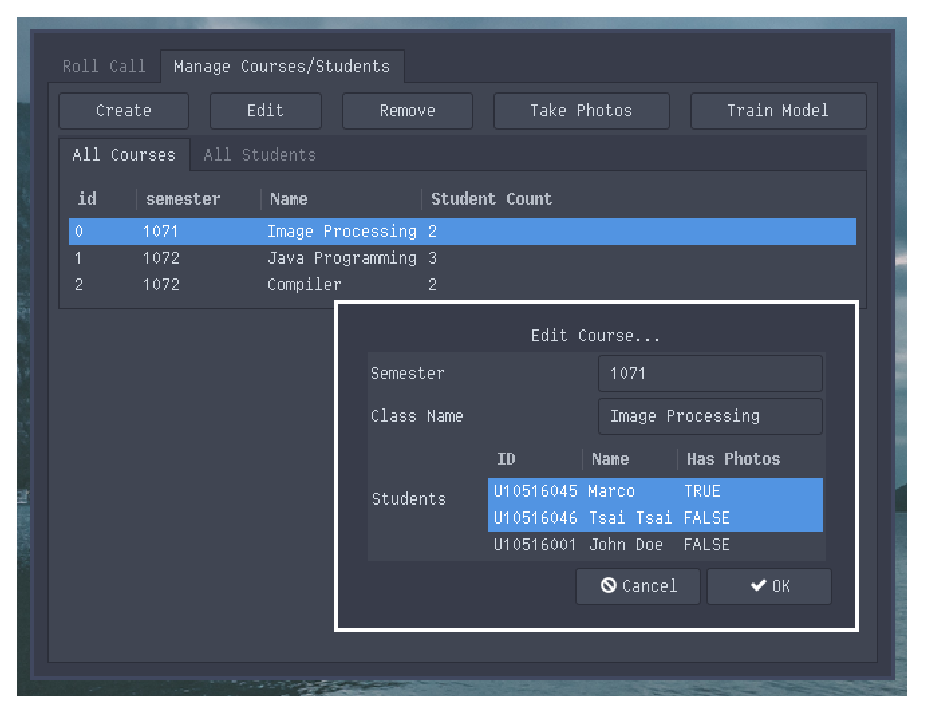
\includegraphics[width=\linewidth]{figures/preview1.eps}
    \caption{Managing courses.}
  \end{subfigure}
  \begin{subfigure}[b]{0.32\linewidth}
    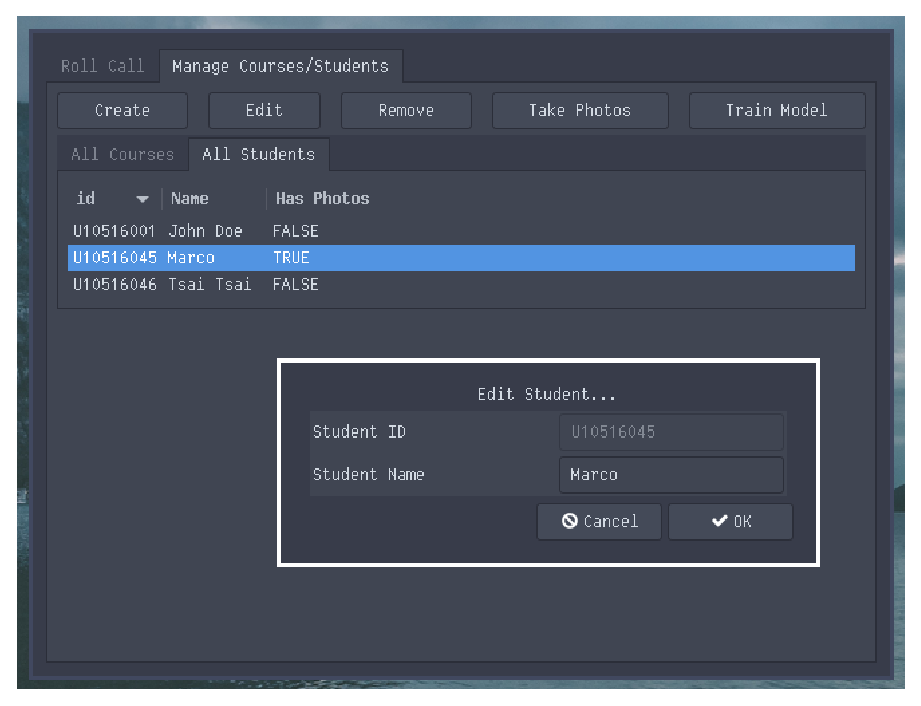
\includegraphics[width=\linewidth]{figures/preview2.eps}
    \caption{Managing students.}
  \end{subfigure}
  \begin{subfigure}[b]{0.32\linewidth}
    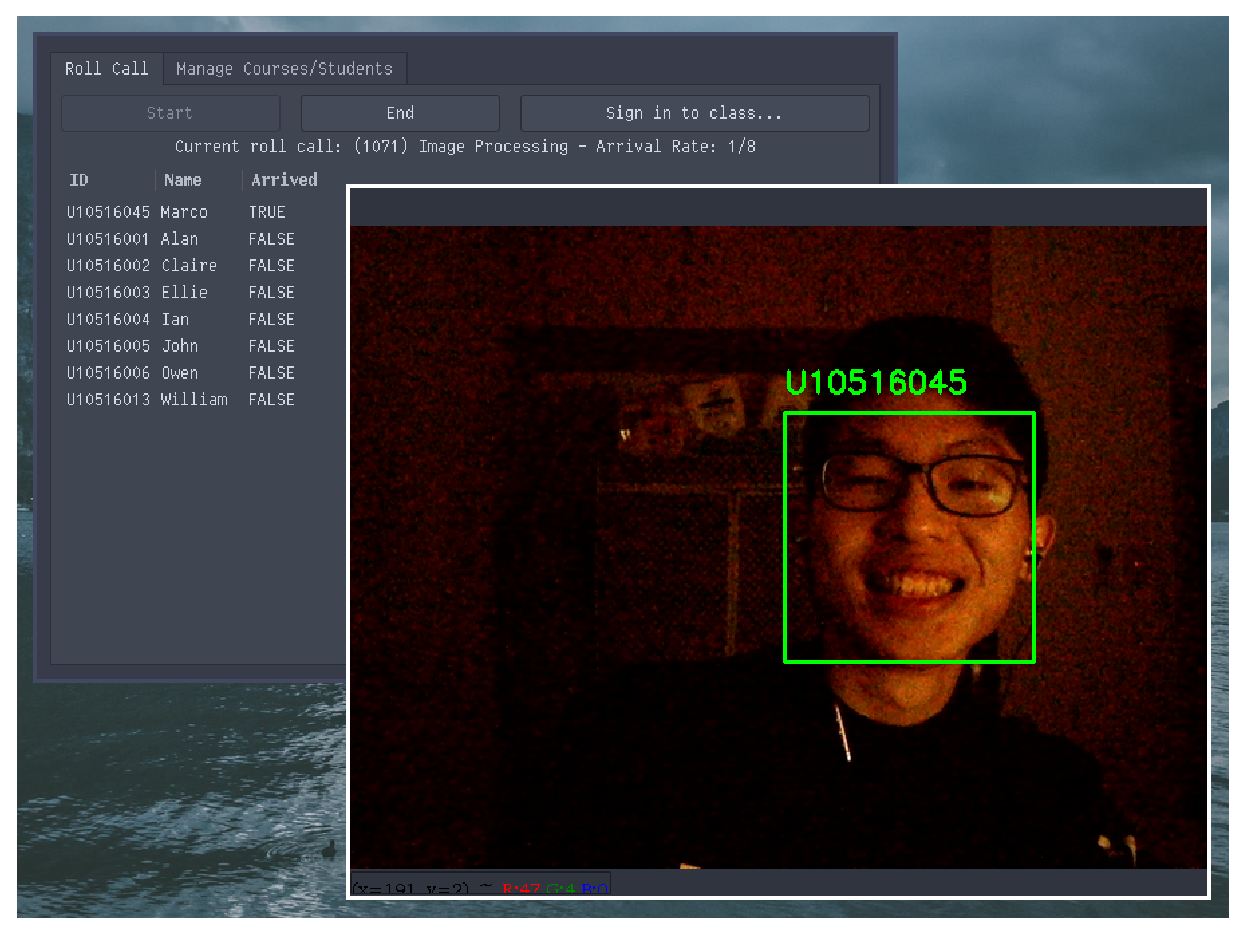
\includegraphics[width=\linewidth]{figures/preview3.eps}
    \caption{A student signing in.}
  \end{subfigure}
  \caption{PyRollCall running on a Linux machine with X11\protect\footnotemark \ installed.}
  \label{fig:systemAppearance}
\end{figure}

\footnotetext{X11, also known as X Window System, or simply X, is a windowing system that provides the basic framework for building GUI environments.}


\subsection{Installation}
Since PyRollCall is cross-platform and all of its external dependencies are already packaged
in the project via Python's \emph{virtualenv}, its installation is fairly simple:

\begin{lstlisting}[numbers=none,xleftmargin=0em,caption={Shell commands to checkout and run PyRollCall}]
$ git clone https://github.com/aesophor/pyrollcall.git
$ cd pyrollcall && ./pyrollcall.py 
\end{lstlisting}

To launch the system, execute \emph{pyrollcall.py}. The Python script can be located at the project's top-level directory.
The system comes with an easy-to-use graphical user interface (GUI) crafted with PyGTK,
allowing teachers to easily
(1) Maintain the data of the course and students they teach,
(2) take photos of students via camera,
(3) train the network with the photos of students,
(4) perform roll calls and
(5) export students' attendance to files.

\begin{algorithm}  
\caption{A}  
\label{alg:A}  
\begin{algorithmic}  
\STATE {set $r(t)=x(t)$}   
\REPEAT   
\STATE set $h(t)=r(t)$   
\REPEAT  
\STATE set $h(t)=r(t)$   
\UNTIL{B}   
\UNTIL{B}  
\end{algorithmic}  
\end{algorithm}  
